\documentclass{article}
\usepackage[utf8]{inputenc}
\usepackage{graphicx}
\graphicspath{ {images/} }
\usepackage{multicol}
\setlength{\columnsep}{2cm}
%\oddsidemargin=0pt % отступ от левого края
%\topmargin=-1.5cm % отступ от верхнего края

\documentclass[12pt]{article}
\usepackage[cp1251]{inputenc}
\usepackage[russian]{babel}
\begin{document}

\begin{titlepage}
	\centering
	{\scshape\LARGE Московский физико-технический институт \par}
	\vspace{3cm}
	{\scshape\Large Лабораторная работа \par}
	\vspace{1cm}
	{\huge\bfseries Исследование стационарного потока жидкости в трубе \par}
	\vspace{1cm}
	%{\Large\itshape John Birdwatch\par}
	\vfill
\begin{flushright}
	{\large выполнили студенты 653 группы ФФКЭ}\par
	\vspace{0.3cm}
	{\LARGE Агафонов Владислав}\\
	{\LARGE Карпова Татьяна} %\textsc{Brown}
\end{flushright}
	

	\vfill

% Bottom of the page
	Долгопрудный, 2017 г.
\end{titlepage}

\section{Цель работы}

\begin{enumerate}
  \item Измерение скорости течения по методам Пито и Вентури
  \item Сравнение результатов со скоростью, определённой по расходу воды.
\end{enumerate}

\section{В работе используются}

\begin{itemize}
  \item расходомерная установка
  \item секундомер
\end{itemize}

\section{Теоретические положения}

Формулы, используемые при расчётах:\\

Уравнение Бернулли для несжимаемой жидкости:

\begin{center}
$ P{}_1{} + \frac {\rho v{}_1{}^2}{2} + \rho gh{}_1{} = P{}_2{} + \frac {\rho v{}_2{}^2}{2} + \rho gh{}_2{} $
\end{center}

Формула Торричелли для истечения струи жидкости из отверстия:
\begin{center}
$ v=\sqrt{2gh} $
\end{center}

Для расходометра Вентури:
\begin{center}
$ v{}_1{}=\sqrt{\frac{2(P{}_1{}-P{}_2{})}{\rho (S{}_1{}/S{}_2{})^2-1}} $
\end{center}

Для расходометра Пито:
\begin{center}
$ v{}_2{}=\sqrt{2(P{}_1{}-P{}_2{})/\rho} $
\end{center}

\section{Схема установки}


\begin{multicols}{2}

\hfill
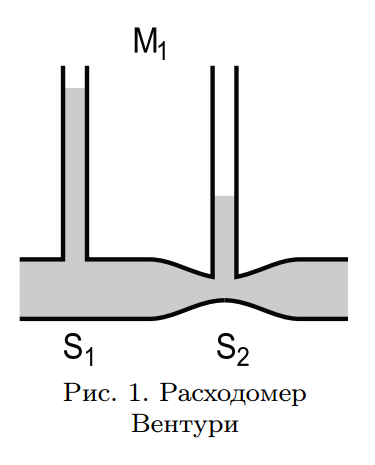
\includegraphics[width=45mm]{ventoury.PNG}
%\hfill
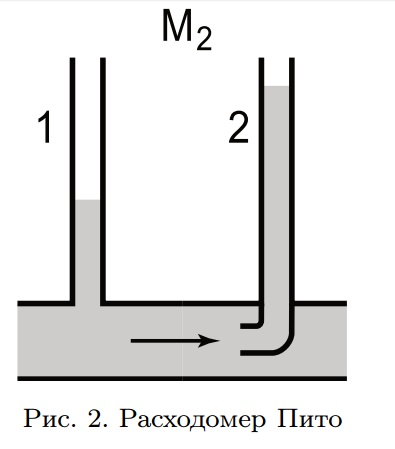
\includegraphics[width=45mm]{pitaux.PNG}
\hfill
\label{figRight}
\end{multicols}

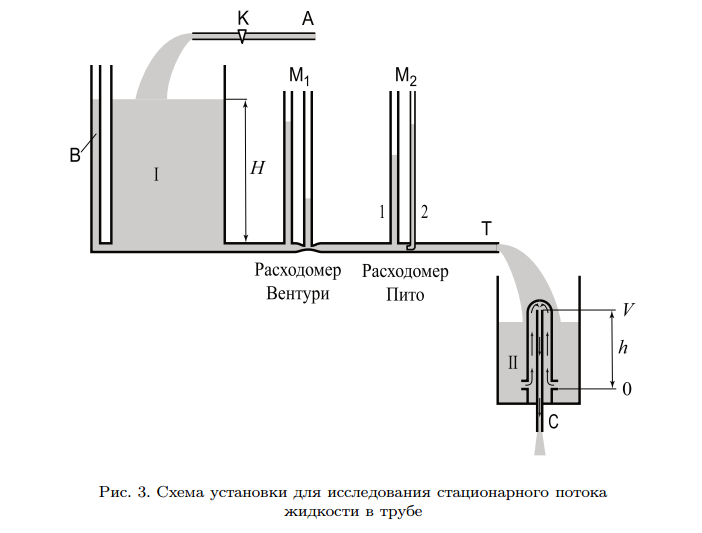
\includegraphics[width=\textwidth]{facility.PNG}

I - цилиндрический резервуар\\
II - приёмный резервуар известного объёма\\
А - водопроводная труба\\
Т - труба с исследуемой водой\\
К - кран для регулировки поступающей воды\\
	\vspace{0.2cm}
С - сифон, автоматически выливающий воду по дистижении ей уровня h\\

Скорость течения, усредненную по сечению трубы, можно опреде-
лить по расходу, который находится по измеренному времени наполне-
ния резервуара II, объем которого задан. С другой стороны, скорость
может быть рассчитана по показаниям манометров. Сопоставление этих скоростей со скоростью, определенной по расходу, позволяет сделать вывод о применимости уравнения Бернулли, роли вязкости, которая, в частности, приводит к изменению скорости поперек потока.
 Для количественной оценки роли вязкости необходимо проделать следующий эксперимент.Установив уровень жидкости в резервуаре I на определенной высоте $z{}_1{}$ измерить скорость течения жидкости по трубе Т с помощью приемного резервуара II (в силу несжимаемости жидкости ее скорость на входе в трубу Т и на выходе из нее одинакова). По измеренному значению
скорости по формуле Торричелли рассчитать ту высоту $z{}_2{}$, при которой жидкость вытекала бы с этой же скоростью в отсутствие вязкости\\
Разность $z{}_1{} - z{}_2{}$ характеризует потери на внутреннее трение в жидкости, причем можно считать, что эти потери происходят только в трубе Т, так как скорость жидкости в резервуаре I существенно меньше.
Влияние вязкости изменяет показания манометра Вентури $\triangle h$ на
величину, которую можно оценить, умножив разность $z{}_1{} - z{}_2{}$ на отношение расстояния между входами манометра $\triangle l$ ко всей длине трубы $L$. При условии
\begin{center}
$\triangle h \geq(z{}_1{} - z{}_2{})\frac {\triangle l}{L}$
\end{center}
неидеальностью жидкости в пределах манометра М можно пренебречь.
В противном случае ($\triangle h$ сравнимо с $z{}_1{} - z{}_2{})\frac {\triangle l}{L}$
 в уравнении для расходомера Вентури из
$p{}_1{} - p{}_2{}$ необходимо вычесть $\triangle z\frac {\triangle l}{L}\rho g$$\\
Аналогично для расходометра Пито

\section{Ход работы}
\begin{enumerate}
\item Проверим исправность установки: после пуска воды закроем конец трубы пробкой. Уровни воды в трубках расходомеров совпали
\item Измерим параметры установки
\begin{multicols}{3}
$L = 222 mm$\\
$\triangle l{}_V{} = 20mm$ \\
%$\triangle l{}_P{} = xxx$
$V= 0,0132 m^3$\\
$S{}_1{}=78.5 cm^3$\\
$D{}_V{}=10mm$ \\
$D{}_P{}=10mm$ \\
$d{}_V{}=6mm$ \\
\end{multicols}
\item Проведём измерения времени заполнения резервуара II для разных уровней H воды в резервуаре I. Результаты занесё в таблицу 1
\begin{table}[h]
    \centering
    \begin{center}
    \caption{Результаты измерения показаний манометров}
    \end{center}
    \vspace{0.1cm}
    \label{tab:my_label}
   \begin{tabular}{ |p{1.5cm}||p{1cm}|p{1cm}|p{1cm}|p{2cm}|p{2cm}|  }
% \multicolumn{12}{|c|}{Country List} \\
 \hline
 $H$, мм & $t{}_1{}$, с & $t{}_2{}$, с & $t{}_3{}$, с & $\triangle h{}_V{}$, мм ($\triangle P{}_V{}$, Па) & $\triangle h{}_P{}$, мм ($\triangle P{}_P{}$, Па)  \\
\hline
 
 100 & 118 & 119 & 118 & 15 & 4 \\
 200 & 79 & 82 & 79 & 35 & 8 \\
 300 & 65 & 70 & 66 & 51 & 12\\
 400 & 55 & 55 & 56 & 67 & 16\\
 500 & 51 & 53 & 50 & 84 & 18\\
 600 & 47 & 45 & 46 & 103 & 21\\
 500 & 54 & 50 & 50 & 84 & 18\\
 400 & 56 & 55 & 55 & 68 & 14\\
 300 & 69 & 65 & 66 & 50 & 12\\
 200 & 84 & 86 & 81 & 33 & 7.5\\
 100 & 119 & 120 & 119 & 16 & 4\\
 \hline
\end{tabular}

\end{table}

\item По среднему времени заполнения резервуара водой вычислим скорость течения воды по расходу $v_p=\frac {V}{tS_1}$. Оценим погрешность определения скорости по формуле $(\frac {\sigma_v}{v})^2=(\frac {\sigma_t}{t})^2+(\frac {\sigma_V}{V})^2+(\frac {\sigma_S}{S})^2$, где $\sigma_t}{t} = \sqrt{\frac{1}{n(n-1)}\sum_{i=1}^n (t_i-\langle x \rangle)^2\quad}$ - погрешность отклонения от среднего, $(\frac {\sigma_V}{V})^2 = (\frac {\sigma_h}{h})^2+(\frac {\sigma_w}{w})^2+(\frac {\sigma_l}{l})^2 = 0.005625m^3 $ , где $h, w, l$ - высота, ширина и длина резервуара II соответственно ($\sigma_w=\sigma_h=\sigma_l = 1cm$ - погрешность линейки) $\sigma_S = 10^-8 m$ - погрешность штангенциркуля
Результаты занесём в таблицу 2
\begin{table}[h]
    \centering
    \begin{center}
    \caption{Расчёт скорости течения по расходу, его погрешность}
    \end{center}
    \vspace{0.1cm}
    \label{tab:my_label}
    \begin{tabular}{ |p{1.5cm}||p{1.5cm}|p{1.5cm}|p{1.5cm}|p{1.5cm}|p{1.5cm}|p{1.5cm}|p{1.5cm}|  }
% \multicolumn{12}{|c|}{Country List} \\
 \hline
 $H, m$ & $t, s$ & $\sigma_t, s$ & $v, m/s$ & $v^2, m^2/s^2$ & $\sigma_v , m/s$ & $\varepsilon, \% $ & $h_t, m^-^3$\\
\hline 

 0,1 & 118,33 & 0,37 & 0,22 & 0,05 & 0,017 & 7,77 & 2,37\\
 0,2 & 80,00 & 1,10 & 0,32 & 0,10 & 0,008 & 2,42 & 5,17\\
 0,3 & 67,00 & 1,67 & 0,38 & 0,14 & 0,012 & 3,20 & 7,38\\
 0,4 & 55,33 & 0,37 & 0,46 & 0,21 & 0,010 & 2,11 & 10,82\\
 0,5 & 51,33 & 0,97 & 0,50 & 0,25 & 0,014 & 2,75 & 12,57\\
 0,6 & 46,00 & 0,63 & 0,55 & 0,31 & 0,013 & 2,43 & 15,65\\
 0,5 & 51,33 & 1,46 & 0,50 & 0,25 & 0,017 & 3,48 & 12,57\\
 0,4 & 55,33 & 0,37 & 0,46 & 0,21 & 0,010 & 2,11 & 10,82\\
 0,3 & 66,67 & 1,32 & 0,38 & 0,15 & 0,011 & 2,81 & 7,45\\
 0,2 & 83,67 & 1,59 & 0,30 & 0,09 & 0,008 & 2,76 & 4,73\\
 0,1 & 119,33 & 0,37 & 0,21 & 0,05 & 0,004 & 2,02 & 2,33\\
 \hline
\end{tabular}

\end{table}
\item Построим график зависимости квадрата скорости от высоты столба жидкости в первом резервуаре. На график нанесём практические значения и теоретическое, где высота столба рассчитана по формуле Торричелли. Погрешности измерения скорости на график наноситьcя не будут, так как они очень малы по сравнению с масштабом всего графика


Наблюдаем несовпадение практического и теоретического значений на два порядка. Возможные причины:
\begin{itemize}
  \item Не учитывалась вязкость воды при расчёте предполагаемой высоты столба
  \item Турбулентный характер движения воды в резервуаре I при его заполнении
  \item То есть, неидеальность жидкости
\end{itemize}
\begin{center}
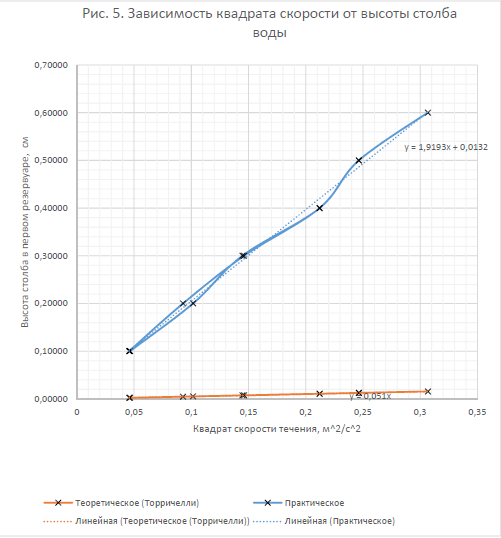
\includegraphics[width=\textwidth]{wrong_torr.PNG}
\end{center}

\item По формулам для расходомеров Вентури и Пито вычислим скорость течения. Сначала вычисления проведём без учёта потерь, затем с ними. Результаты занесём в таблицу 3.

В уравнении для расходомера Вентури из
$p{}_1{} - p{}_2{}$ необходимо вычесть $\triangle z\frac {\triangle l}{L}\rho g$\\
Для расходомера Пито проведём следующую оценку\\
Скорость жидкости в центре трубы по формуле Пуазейля:
\begin{center}
$v_0 =\frac{1}{4\nu}\frac{\triangle P}{L}(R^2)$
\end{center}
Скорость жидкости у края трубки расходомера Пито:\\
\begin{center}
$v(r) =\frac{1}{4\nu}\frac{\triangle P}{L}(R^2-r^2)$
\end{center}
Средняя скорость в трубке Пито:\\
\begin{center}
$v_P =\frac{1}{4\nu}\frac{\triangle P}{L}(R^2-\frac{r^2}{2})$
\end{center}
Тогда\\
\begin{center}
$\frac{1}{4\nu}\frac{\triangle P}{L}) =\frac{v_0}{R^2}$
\end{center}
Окончательно средняя скорость воды в трубе:\\
\begin{center}
$v_0 =\frac{v_P R^2}{R^2-\frac{r^2}{2}}$
\end{center}

\begin{table}[h]
    \centering
    \begin{center}
    \caption{Скорости по расходу и по расходомерам}
    \end{center}
    \vspace{0.1cm}
    \label{tab:my_label}
   \begin{tabular}{ |p{1.5cm}|p{1.5cm}|p{1.5cm}|p{1.5cm}|p{1.5cm}|  }
 \hline
 $v_p$, м/с & $v_V_e_n_t$, м/с & $v_P_i_t_o_t$, м/с & $v*_V_e_n_t$, м/с & $v*_P_i_t_o_t$, м/с   \\
\hline
0,215 & 0,209 & 0,280 &	0,264 &	0,304\\
0,318 & 0,320 &	0,396 &	0,392 &	0,430\\
0,380 & 0,386 &	0,485 &	0,475 &	0,527\\
0,460 & 0,442 &	0,560 &	0,546 &	0,609\\
0,496 & 0,495 &	0,594 &	0,611 &	0,646\\
0,554 & 0,548 &	0,642 &	0,674 &	0,697\\
0,496 & 0,495 &	0,594 &	0,611 &	0,646\\
0,460 & 0,445 &	0,524 &	0,548 &	0,569\\
0,382 & 0,382 &	0,485 &	0,472 &	0,527\\
0,305 & 0,310 &	0,383 &	0,384 &	0,417\\
0,214 & 0,216 &	0,280 &	0,269 &	0,304\\
\hline
\end{tabular}

\end{table}

Для наглядности представим зависимость этих значений от значения скорости по расходу на одном графике (рисунок 5).

\begin{center}
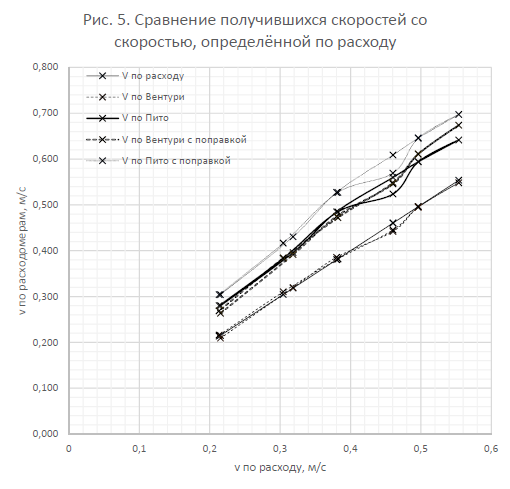
\includegraphics[width=\textwidth]{velocities.PNG}
\end{center}
Видим, что примерно одинаковыми оказались скорости, определённые по расходу и по расходомеру Вентури, по расходомеру Пито и по расходомеру Вентури с поправкой. Истинная скорость движения жидкости самая малая среди всех определённых скоростей, так как при их расчёте мы не учитывали вязкость жидкости, снижающую скорость.\\

\item Построим график зависимости скорости течения по расходу от высоты столба воды (рисунок 6)

\begin{center}
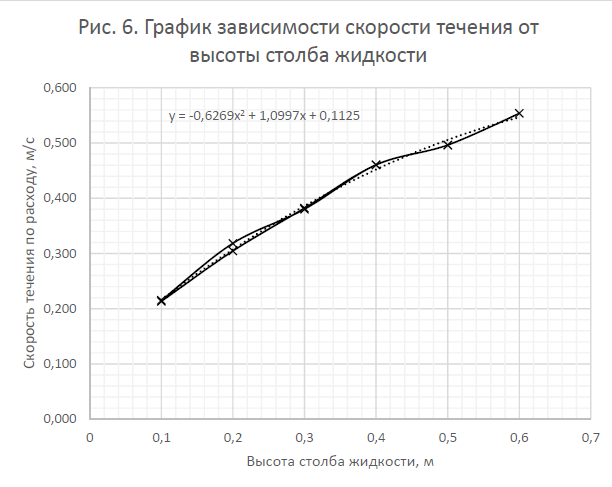
\includegraphics[width=\textwidth]{raynolds.PNG}
\end{center}

По графику определим участки ламинарного и турбулентного течений. Вычислим значение числа Рейнольдса для точки, в которой теряется линейный характер графика: на третьей точке при $v = 0.380$ м/с определим число Рейнольдса по формуле $Re = \frac{v_pR\rho}{\eta} = 1900$. В справочниках указано, что в трубе круглого сечения переход течения воды при комнатной температуре из ламинарного в турбулентный режим происходит при $Re \approx 1800$.
Убедимся, что при меньших чем граничая точка значениях скорости число Рейнольдса $\loe 1000$, а при больших > 2000:\\
\begin{center}
$Re(0.215) = 1075$\\
$Re(0.554) = 2770$\\
\end{center}
Теоретическая скорость, когда течение станет турбулентным: $v = 0.360$м/с
Итак, наша оценка верна. Стоит отметить, что при достижении достаточно больших скоростей в трубе наблюдалось образование пузырьков жидкости, что также является признаком турбулентного течения жидкости

\end{enumerate}

\section{Вывод}

В ходе работы было исследовано течение жидкости в цилиндрической трубе, изучен принцип работы расходомеров Вентури и Пито, исследованы ламинарный и стационарный режимы течения жидкости. 
\begin{itemize}
  \item По расходу жидкости была определена зависимость квадрата скорости воды от высоты столба воды в резервуаре I: чётко прослеживается линейный характер
  \item Выяснено, что использование уравнения Торричелли для расчёта столба жидкости по скорости её течения неуместна по причине того, что рассматривается реальная, а не идеальная жидкость. Учитывая явно турбулентный характер движения жидкости в резервуаре при его заполнении, использование любых формул для ламинарного истечения из него бессмысленно
  \item Исследованы расходомеры Пито и Вентури, определены поправки для более точного расчёта скорости воды по их показаниям. Выяснилось, что наиболее точным является расходомер Вентури. Расходомер Пито показывает повышенное значение скорости, так как его трубка расположена в центре потока (пуазейлевкий профиль скоростей в реальной жидкости). Для более точных измерений с помощью расходомера Пито необходимо использовать несколько расходомеров, расположив их на разных расстояниях он центра трубы и усреднив полученные значения.
  \item По графику зависимости скорости течения от высоты столба жидкости определены участки ламинарного и турбулентного течения воды, найдена точка, в которой предположительно течение меняет характер с ламинарного на турбулентное; эмпирически и теоретически подтверждено что при больших скоростях течение имеет турбулентный характер.
\end{itemize}

\end{document}

